%\TODO{the annotation of tuples is encoded as an attribute in implementation.}
%\TODO{fix the fig}
%
%\point{vdb and vschema and config (bottom of fig).}
%\textbf{VDBMS architecture:}
\figref{arch} shows the architecture of VDBMS and its modules.
The implantation of VDB directly follows its formalization given in 
\secref{vtab}. The only difference is that the presence conditions
of a tuple is encoded as an extra attribute in the underlying relational
database. 
For now, we assume a VDB and its v-schema are generated by an 
expert and are stored in a DBMS, we provide guidelines and case studies of
systematically generating VDBs in 
\secref{db}. A VDB can be \emph{configured} to its pure relational 
database variants, if desired by a user, by providing the configuration
of the desired variant, \figref{vdb-conf}.
For example, a SPL developer configures a VDB to produce 
software and its database for a client.
%To configure a VDB, VDBMS requires a list of valid configurations.
%Remember that the feature model is a feature expression that 
%encodes all valid configurations. Hence, solving the feature model
%by a SAT solver results in the list of valid configurations.

%\point{flow of vq in vdbms.}
Given a VDB and its v-schema, a user inputs a v-query \vQ\ to VDBMS.
%
First, \vQ\ is checked by the \emph{type system} to determine if it is invalid, explained in 
%First, \vQ\ is type-checked by the VRA type system introduced in 
\secref{type-sys}. 
If so, the user gets errors explaining what part of the 
query violated the v-schema.
%, shown in \exref{q-violate-sch}.
%\moredet{maybe give an ex of an error user will see! ref to ex of error given
%in \secref{type-sys}}
Otherwise, 
\vQ\ is explicitly annotated with the schema,
defined in \secref{constrain},
to ensure variation-preserving property w.r.t. v-schema throughout the execution flow of v-query 
in the system and then
%
it is passed to the \emph{variation minimization} module, introduced in 
\secref{var-min}, to minimize the variation of \vQ\ and apply
relational algebra optimization rules. 
%
The optimized query is then sent to the \emph{generator} module where
SQL queries are generated from v-queries using one of the following approaches:
%, \secref{apps} provides three
%approaches for this.
%\exref{q-flow} in \appref{sql-gen} demonstrates the flow of a v-query through
%VDBMS.
\begin{enumerate}
%[wide, labelwidth=!, labelindent=0pt, topsep=1pt]
%\itemsep0em
\item
\emph{Naive Brute Force (\nbf):}
Configures a v-query \vQ\ for all valid configurations, i.e., 
\ensuremath{\forall \config \in \confSet}, translates them to RA queries,
and finally generates SQL queries with renaming all subqueries. The 
SQL queries are sent to underlying DBMS and the results are gathered and
cleaned up in v-table builder module. Here is the flow of how results are generated by 
this approach:
%
\[\vQ \mathrel{\mathop{\rightarrow}^{\mathrm{\eeSem \vQ}}} [ ( \config, \pQ ) ] 
\mathrel{\mathop{\rightarrow}^{\mathrm{\textit{translate}}}_{\mathrm{\textit{to SQL}}}} [ ( \config, \sqlQ ) ]
\mathrel{\mathop{\rightarrow}^{\mathrm{\textit{run}}}_{\mathrm{\textit{queries}}}} \textit{v-tables}
\mathrel{\mathop{\rightarrow}^{\mathrm{\textit{v-table}}}_{\mathrm{\textit{builder}}}} \textit{v-table}
\]

\item
\emph{Unique Brute Force (\ubf):}
This approach is just like \nbf\ except that we only generate SQL 
queries for unique RA queries which are the result of configuring the v-query.
The trick is to attach the condition under which a 
RA query is valid. This condition is a feature expression generated from
the set of configurations that configured the v-query into the same RA query, i.e.,
\ensuremath{
\qGroup \vQ = \setDef {\annot \pQ \myOR \forall \config \in \confSet: \fSem \dimMeta = \t,
\eeSem \vQ = \pQ}
}. The implementation of this function is more efficient than its definition.
That is:
%Groups variants of a v-query, translates them to RA queries,
%and generates SQK queries with renaming subqueries. Similar to 
%\ensuremath{(1)} results are gathered and cleaned up by v-table builder module.
%Here is the flow of how results are generated by 
%this approach:
%
\[\vQ \mathrel{\mathop{\rightarrow}^{\mathrm{\qGroup \vQ}}} [ \annot [\dimMeta] {\pQ} ] 
\mathrel{\mathop{\rightarrow}^{\mathrm{\textit{translate}}}_{\mathrm{\textit{to SQL}}}} [ \annot [\dimMeta] {\sqlQ} ]
\mathrel{\mathop{\rightarrow}^{\mathrm{\textit{run}}}_{\mathrm{\textit{queries}}}} \textit{v-tables}
\mathrel{\mathop{\rightarrow}^{\mathrm{\textit{v-table}}}_{\mathrm{\textit{builder}}}} \textit{v-table}
\]

\item
\emph{Union-All-Variants (\uav):}
This approach takes the SQL queries generated by \ubf\ and 
unions them to just run one SQL query. In order to do so it 
forces all the SQL queries to return the same set of attributes.
Additionally, it applies the presence condition of a SQL query
to its tuples by concating it with the presence condition attribute
in the projected attribute set.
%Groups variants of a v-query, translates them to RA queries, 
%translates RA queries to SQL queries, 
%%generates one SQL query from all SQL queries by u
%unifies the set of
%attributes returned by SQL queries (by getting all returned attributes from
%the type of the v-query and for an attribute \vAtt\ that a SQL query is not returning,
%it uses \ensuremath{\mathbf{NULL} \textit{\ } \mathbf{AS} \textit{\ } \vAtt} syntax),
%attaches the presence condition of variant SQL queries to them (by concating the
%feature expression with presence condition attribute in the returned attribute set),
%%, i.e., 
%%\ensuremath{\mathbf{presenceCond} \textit{\ }  
%and finally combines SQL queries by set operation union. 
The query is sent to the underlying
DBMS and result is cleaned up and returned to the user as a v-table. Note that cleaning up
the result is part of v-table builder tasks.
%% by attaching presence 
%%condition of attributes to them. 
%Here is the flow of how results are generated by 
%this approach:
That is:
%
\[\vQ \mathrel{\mathop{\rightarrow}^{\mathrm{\qGroup \vQ}}} [ \annot [\dimMeta] {\pQ} ] 
\mathrel{\mathop{\rightarrow}^{\mathrm{\textit{generate}}}_{\mathrm{\textit{SQL}}}} [ \annot [\dimMeta] {\sqlQ} ]
\mathrel{\mathop{\rightarrow}^{\mathrm{union}}} {\VVal \sqlQ}
\mathrel{\mathop{\rightarrow}^{\mathrm{\textit{run}}}_{\mathrm{\textit{query}}}} \textit{v-table}
\mathrel{\mathop{\rightarrow}^{\mathrm{\textit{clean up}}}} \textit{v-table}
\]

\end{enumerate}

We use these
SQL generators to simulate current approaches used to manage
variation currently. In particular, \nbf\ simulates how a naive
DBA would conduct such a task. \ubf\ simulates
how an expert DBA would conduct such a task. 
The generated SQL queries need to be independent from the 
underlying DBMS that stores the VDB. Hence, the SQL generator module
has a submodule that prints generated SQL queries for each DBMS engine. 


\begin{comment}
To generate runnable queries w.r.t. the underlying DBMS,
the minimized query \ensuremath {\VVal \vQ} is passed to 
the \emph{translate to RA} module that could use either 
configuring or grouping of v-queries, explained in \secref{vra-sem},
to generate RA queries. The generated 
queries are then sent to the \emph{SQL generator} module which generates
SQL queries in various ways from the relational algebra queries, explained
in \secref{sql-gen}.
%\moredet{in app have an ex of all this happening!}
\end{comment}

%\point{vtab builder.}
Having generated SQL queries, they are now run over the underlying 
VDB (stored in a DBMS desired by the user). The result could be either 
a v-table or a list of v-tables, depending on the approach chosen in 
the translator to RA and SQL generator modules. The v-table(s) is passed
to the \emph{v-table builder}
%\dropit{could drop \secref{vtab-build} and explain it here!}
%explained in \secref{vtab-build}, 
to create one v-table that filters out 
duplicate and invalid tuples, shrinks presence conditions, and 
eventually, returns the final v-table to the user.

\begin{figure}
\centering
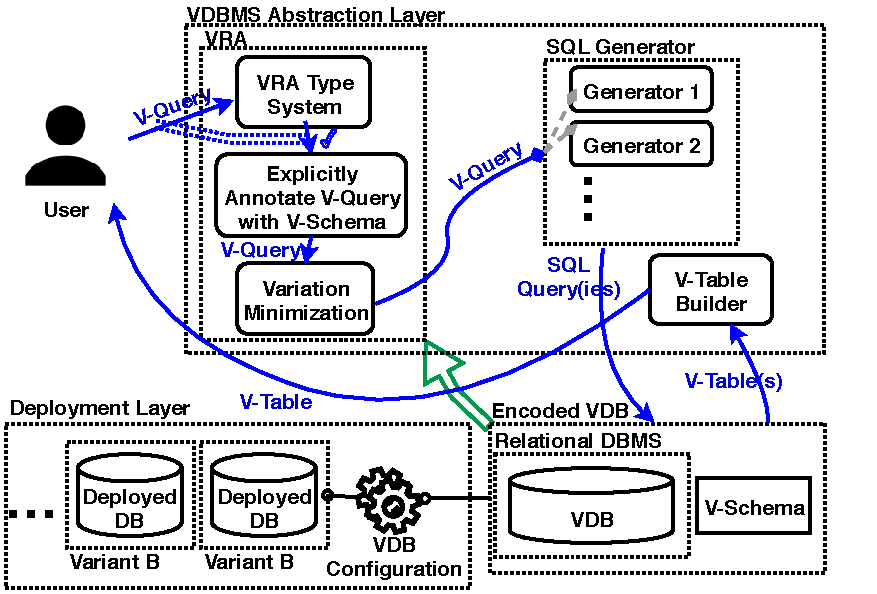
\includegraphics[scale = 0.7] {figs/arch8.pdf}
\caption{VDBMS architecture and execution flow of a v-query. 
The dotted double-line from v-query to pushing v-schema module
indicates the dependency of passing the v-query to this module
only if it is valid. 
The dashed gray arrows with diamond heads demonstrate
an option for the flow of input. 
%We examine taking different routes
%to evaluate a v-query, resulting in various approaches in \secref{apps}.
The blue filled arrows track the data flow, the green hollow arrows 
indicate an input to a module.}
\label{fig:arch}
\end{figure}


